\documentclass[10pt]{article}
\usepackage{fourier}
\usepackage[hmargin=2cm,vmargin=2.5cm]{geometry} % see geometry.pdf on how to lay out
%\usepackage{fullpage}
\usepackage{graphicx}
\usepackage{tabularx}
\usepackage{multirow}
%\usepackage{subfigure}

\usepackage{float}
\usepackage{caption}
\usepackage{amssymb,amsmath}
%\usepackage{bbm} 
\usepackage{hyperref}
\usepackage{enumitem}
\geometry{letterpaper} % a4paper or letter or a5paper or ... etc
\linespread{1.1}% \geometry{landscape} % rotated page geometry
\usepackage{pythonhighlight}
\setcounter{MaxMatrixCols}{14}
\usepackage{subcaption}

\title{\huge CE 295 PROGRESS REPORT}


\author{
$\begin{array}{rl}
\text{Xin Peng}&\href{mailto:xin-peng@berkeley.edu}{(\textsc{xin-peng@berkeley.edu})}\\
\text{Junzhe Shi}&\href{mailto:junzhe@berkeley.edu}{(\textsc{junzhe@berkeley.edu})}\ \ \ \\
\text{Franklin Zhao}&\href{mailto:qingan_zhao@berkeley.edu}{(\textsc{qingan\_zhao@berkeley.edu})}\\
\text{Ruitong Zhu}&\href{mailto:ruitong_zhu@berkeley.edu}{(\textsc{ruitong\_zhu@berkeley.edu})}
\end{array}$
}
\date{18 Mar. 2018} 
\begin{document}

\maketitle

\renewcommand{\theequation}{\arabic{equation}}
%\newcommand{\tabincell}[2]{\begin{tabular}{@{}#1@{}}#2\end{tabular}}
\renewcommand{\figurename}{Fig.}
%\renewcommand\thesection{\Roman{section}}
\renewcommand\thesubsection{(\alph{subsection})}
\renewcommand\thesubsubsection{\Roman{subsubsection}}

\noindent \textbf{Abstract:} Batteries are ubiquitous in all forms of electronics and transportation, and also are a key to the store of clean and secure energy. In different kinds of batteries,  Li-ion battery is the most prominent one due to their superior gravimetric and volumetric energy density.  For the safe operation of Li-ion battery, the state of charge (SOC) and state of health (SOH) estimation is of great significance. Hence, the goal of the project is to design a robust observer which can estimate the SOC and SOH of Li-ion batteries. \textbf{So far, based on the research of Perez et al. \cite{ref:1}, we have successfully established the electrical model, thermal model, and aging model. Ambient temperature is novelly considered as an uncontrollable input in our project. The open-loop simulation is also implemented in this report.}\\\\
\textbf{Keywords:} Battery; SOC; SOH; Open-loop simulation  
\section{Introduction}
The identification of battery operation and aging in real life has been a long-desired yet challenging goal, which includes multiple complex processes in complicated operating conditions and environments. An accurate method to observe SOC and SOH of Li-ion battery is in need. Meanwhile, batteries invariably work at varying thermal and aging conditions. Thus, it is necessary for us to build a battery observation system to monitor operation and aging of battery. In this project, we will focus on the SOC and SOH of LI-ion batteries. Based on equivalent-circuit, the electrical, thermal and aging models will be developed for the observing system. Since battery monitoring and management can be the key to allowing innovation in future designs because of their limit properties, our system may play an important role in such an area, and significantly contribute to the energy saving and efficiency. 
\section{Technical Description}
\subsection{Mathematical Model}
Our analysis is based on a coupled electro-thermal-aging model for lithium-iron-phosphate batteries, which is introduced in \cite{ref:1}. 
The model consists of a two RC pair electrical model, a two-state thermal model and a semi-empirical aging model.
\subsubsection{Electrical Model}
As shown in Figure \ref{p1}, the electrical comprises an open-circuit voltage $(OCV, V_{OC})$, two resistor-capacitor (RC) pairs ($R_1$, $C_1$, $R_2$, $C_2$), and an ohmic resistor ($R_0$). The state-space model is given by:
\begin{equation}
	\frac{\mathrm{d} SOC}{\mathrm{d}t}(t) = \frac{I(t)}{C_{bat}}
\end{equation}
\begin{equation}
\frac{\mathrm{d} V_1}{\mathrm{d}t}(t) = -\frac{V_1(t)}{R_1C_1}+\frac{I(t)}{C_1}
\end{equation}
\begin{equation}
\frac{\mathrm{d} V_2}{\mathrm{d}t}(t) = -\frac{V_2(t)}{R_2C_2}+\frac{I(t)}{C_2}
\end{equation}
\begin{equation}
V_t(t) = V_{OC}(SOC)+V_1(t)+V_2(t)+R_0I(t)
\end{equation}
where $C_{bat}$ is the nominal capacity of the battery, $I(t)$ is the current (positive for charging), and $V_t(t)$ denotes the terminal voltage. Three state variabels are $SOC$ and volatges across the two RC pairs $V_1$, $V_2$. 
\begin{figure}[H]
	\centering
	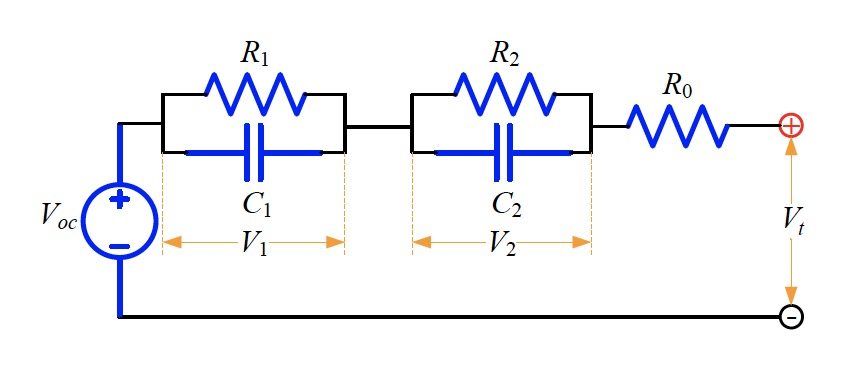
\includegraphics[height=0.3\textwidth]{circuit.jpg}
	\caption{Electrical Model}
	\label{p1}
\end{figure}
\noindent The electrical parameters are identified in \cite{ref:1}. In our model, we follow the equations shown to derive these parameters based on the state of charge ($I<0$) or discharge ($I\ge 0$).
\begin{equation}
R_{1} = \begin{Bmatrix}
R_{1d}&I\ge 0\\
R_{1c} &I<0
\end{Bmatrix}    
\end{equation}
\begin{equation}
R_{1_{*}}=(R_{10_{*}}+R_{11_{*}}(SOC)+R_{12_{*}}(SOC)^{2})exp\left ( \frac{T_{refR_{1}*}}{T_m-T_{shiftR_{1}*}} \right )
\end{equation}
\begin{table}[H]
	\caption{PARAMETRIC \ $R_1$ \ FUNCTION PARAMETERS}
	\vspace{-0.4cm}
	\centering
	\begin{tabular}{lllll}
		\hline
		$R_{10_{d}}$ & $R_{10_{c}}$ & $R_{11_{d}}$ & $R_{11_{c}}$ &$R_{12_{d}}$  \\
		\hline
		7.1135e-4 & 0.0016 & -4.3865e-4 & -0.0032 & 2.3788e-4 \\
		\hline
		$R_{12_{c}}$ & $T_{refR_{1}d}$& $T_{refR_{1}c}$ &$T_{shiftR_{1}d}$ & $T_{shiftR_{1}c}$\\
		\hline
		0.0045 & 347.4707 & 159.2819 & -79.5816 & -41.4578 \\
		\hline
	\end{tabular}
\end{table}
\begin{equation}
R_{2} = 
\begin{Bmatrix}
R_{2d}&I\ge 0\\
R_{2c} &I<0
\end{Bmatrix}
\end{equation}
\begin{equation}
R_{2_{*}}=(R_{20_{*}}+R_{21_{*}}(SOC)+R_{22_{*}}(SOC)^{2})exp\left ( \frac{T_{refR_{2}*}}{T_m} \right )
\end{equation}
\begin{table}[H]
	\caption{PARAMETRIC \ $R_2$ \ FUNCTION PARAMETERS}
	\vspace{-0.4cm}
	\centering
	\begin{tabular}{llll}
		\hline
		$R_{20_{d}}$ & $R_{20_{c}}$ & $R_{21_{d}}$ & $R_{21_{c}}$ \\
		\hline
		0.0288 & 0.0113 & -0.073 & -0.027  \\
		\hline
		$R_{22_{d}}$ & $R_{22_{c}}$& $T_{refR_{2}d}$& $T_{refR_{2}c}$ \\
		\hline
		0.0605 & 0.0339 & 16.6712 & 17.0224 \\
		\hline
	\end{tabular}
\end{table}
\begin{equation}
C_{1} = 
\begin{Bmatrix}
C_{1d}&I\ge 0 \\
C_{1c} &I<0
\end{Bmatrix}
\end{equation}
\begin{equation}
C_{1_{*}}=C_{10_{*}}+C_{11_{*}}(SOC)+C_{12_{*}}(SOC)^{2}+(C_{13_{*}}+C_{14_{*}}(SOC)+C_{15_{*}}(SOC)^{2}){T_m}
\end{equation}
\begin{table}[H]
	\caption{PARAMETRIC \ $C_1$ \  FUNCTION PARAMETERS}
	\vspace{-0.4cm}
	\centering
	\begin{tabular}{llll}
		\hline
		$C_{10_{d}}$ & $C_{10_{c}}$ & $C_{11_{d}}$ & $C_{11_{c}}$ \\
		\hline
		335.4518 & 523.215 & 3.1712e+3 & 6.4171e+3  \\
		\hline
		$C_{12_{d}}$ & $C_{12_{c}}$ & $C_{13_{d}}$ & $C_{13_{c}}$ \\
		\hline
		-1.3214e+3 & -7.5555e+3 & 53.2138 & 50.7107 \\
		\hline
		$C_{14_{d}}$ & $C_{14_{c}}$ & $C_{15_{d}}$ & $C_{15_{c}}$ \\
		\hline
		-65.4786 & -131.2298 & 44.3761 & 162.4688 \\
		\hline
	\end{tabular}
\end{table}
\begin{equation}
C_{2} = 
\begin{Bmatrix}
C_{2d}&I\ge 0  \\
C_{2c} &I<0
\end{Bmatrix}
\end{equation}
\begin{equation}
C_{2_{*}}=C_{20_{*}}+C_{21_{*}}(SOC)+C_{22_{*}}(SOC)^{2}+(C_{23_{*}}+C_{24_{*}}(SOC)+C_{25_{*}}(SOC)^{2}){T_m}
\end{equation}
\begin{table}[H]
	\caption{PARAMETRIC \ $C_1$ \ FUNCTION PARAMETERS}
	\vspace{-0.4cm}
	\centering
	\begin{tabular}{llll}
		\hline
		$C_{20_{d}}$ & $C_{20_{c}}$ & $C_{21_{d}}$ & $C_{21_{c}}$ \\
		\hline
		3.1887e+4 & 6.2449e+4 & -1.1593e+5 & -1.055e+5  \\
		\hline
		$C_{22_{d}}$ & $C_{22_{c}}$ & $C_{23_{d}}$ & $C_{23_{c}}$ \\
		\hline
		1.0493e+5 & 4.4432e+4 & 60.3114 & 198.9753 \\
		\hline
		$C_{24_{d}}$ & $C_{24_{c}}$ & $C_{25_{d}}$ & $C_{25_{c}}$ \\
		\hline
		1.0175e+4 & 7.5921e+3 & -9.5924e+3 & -6.9365e+3 \\
		\hline
	\end{tabular}
\end{table}
\subsubsection{Thermal Model}
\begin{figure}[H]
	\centering
	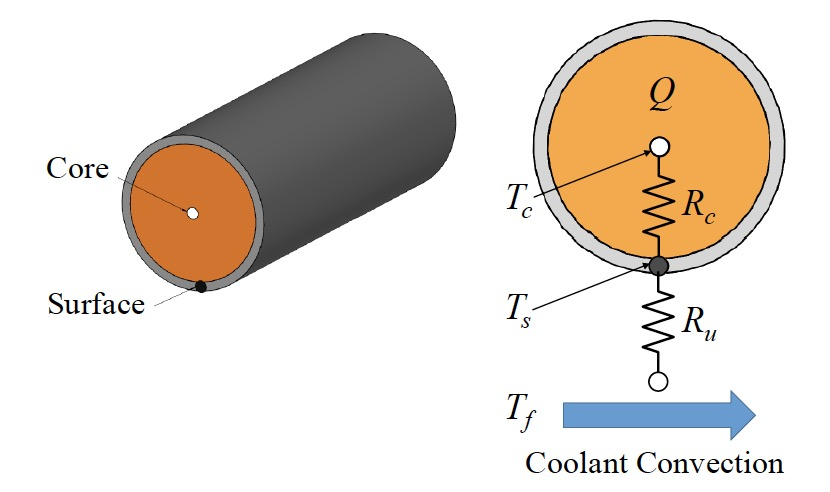
\includegraphics[height=0.3\textwidth]{thermal.jpg}
	\caption{Two-state Thermal Model}
	\label{p2}
\end{figure}
Since the core tempturature can be higher than the surface temperature under high current rates \cite{ref:2}, a two-state thermal system was hereby intruduced to capture both core and surface temperature dynamics. As sketched in Figure \ref{p2}, the radial heat transfer dynamics of a cylindrical battery can be described as follow.
\begin{equation}
	\frac{\mathrm{d}T_c(t)}{\mathrm{d} t} = \frac{T_s(t)-T_c(t)}{R_cC_c}+\frac{Q(t)}{C_c}
\end{equation}
\begin{equation}
\frac{\mathrm{d}T_s(t)}{\mathrm{d} t} = \frac{T_f(t)-T_s(t)}{R_uC_s}+\frac{T_s(t)-T_c(t)}{R_cC_s}
\end{equation}
$R_c$, $R_u$, $C_c$ and $C_s$ represent the heat conduction resistance, convection resistance, core heat capacity and surface heat capacity respectively, with their values shown in Table \ref{t5}; two state variables are core temperature $T_c$ and surface temperature $T_s$; the ambient temperature $T_f$ is treated as uncontrollabel input. 
\begin{table}[H]
	\caption{THERMAL PARAMETERS}
	\vspace{-0.4cm}
	\centering
	\begin{tabular}{llll}
		\hline
		$R_{c}(KW^{-1})$ & $R_{u}(KW^{-1})$ & $C_{c}(JK^{-1})$ & $C_{s}(JK^{-1})$ \\
		\hline
		1.94 & 3.08 & 62.7 & 4.5  \\
		\hline
	\end{tabular}
    \label{t5}
\end{table}
\noindent $Q(t)=|I(V_{OC}-V_t)|$ is heat generation including joule heating and energy dissipated by electrode over-potentials, based on equation (4), we can rewrite equation (5) as
\begin{equation}
\frac{\mathrm{d}T_c(t)}{\mathrm{d} t} = \frac{T_s(t)-T_c(t)}{R_cC_c}+\frac{I(t)(V_1(t)+V_2(t)+R_0I(t)}{C_c}
\end{equation}
\subsubsection{Aging Model}
The aging model is based upon a matrix of cycling tests from \cite{ref:3}. The experiment results suggest that capacity fade depends strongly on C-rate and temperature in the cell at low charge'discharge rates, while the sensitivity to depth-of-discharge is negligible. The semi-empirical life model adopted the following equation to describe the correlation between the capacity loss ($\Delta Q_b$, in $\%$) and the discharged Ah throughput($A$, depends on C-rate),
\begin{equation}
	\Delta Q_b = M(c)\mathrm{exp}\left(\frac{-E_a(c)}{RT_c}\right)A(c)^z
\end{equation}
where $M(c)$ is the pre-exponential factor as a funciton of C-rate, which is denoted by $c$. The relation between the pre-exponential factor $M(c)$ and C-rate are shown in Table \ref{t6}. The activation energy $E_a$ and the power-law factor $z$ are given by
\begin{equation}
	E_a(c)=31700-370.3c  \quad z=0.55
\end{equation}
\begin{table}[H]
	\caption{PRE-EXPONENTIAL FACTOR AS A FUNCTION OF THE C-RATE}
	\vspace{-0.4cm}
	\centering
	\begin{tabular}{lllll}
		\hline
		C-rate c & 0.5 & 2 & 6 & 10 \\
		\hline
		M & 31630 & 21681 & 12934 & 15512  \\
		\hline
	\end{tabular}
\label{t6}
\end{table}
\noindent The model consider a capacity loss of $20\%$ as the end-of-life (EOL) for an automotive battery. The corresponding Ah throughput $A_{tol}$ and the number of cycles $N$ are therefore calculated as below.
\begin{equation}
A_{tol} (c, T_c) = \left[ \frac{20}{M(c)\mathrm{exp}\left(\frac{-E_a(c)}{RT_c}\right)} \right]^{\frac{1}{z}}
\end{equation}
\begin{equation}
N(c, T_c) = \frac{3600A_{tol} (c, T_c) }{C_{bat}}
\end{equation}
Each cycle correspondes to $2C_{bat}$ charge throughput, and since $A_{tol}$ is discharged Ah throughput, the total throughput including both charged and discharged Ah should be $2A_{tol}$. Based on this, the battery State-of-Health (SOH) is defined as: 
\begin{equation}
SOH(t) = SOH(t_0)-\frac{\int_{t_0}^{t}|I(\tau)\mathrm{d}\tau}{2N(c, T_c) C_{bat}}
\end{equation}
where $t_0$ denotes the initial time. $SOH$ varies among $[0,1]$, $SOH=1$ correspondes to a brand new battery and $SOH=0$  means $20\%$ capacity loss, as known as EOL. The derivative of $SOH$ yields the battery aging model
\begin{equation}
	\frac{\mathrm{d} SOH}{\mathrm{d}t}(t) = -\frac{|I(t)|}{2N(c, T_c) C_{bat}}
\end{equation}
\subsection*{(b) Simulation}
The simulation is based on a 2.3Ah A123 26650 LiFePO4 battery as described in \cite{ref:1}, with simulation duration to be 2 hours (7200s) in total.
\begin{figure}[H]
	\centering
	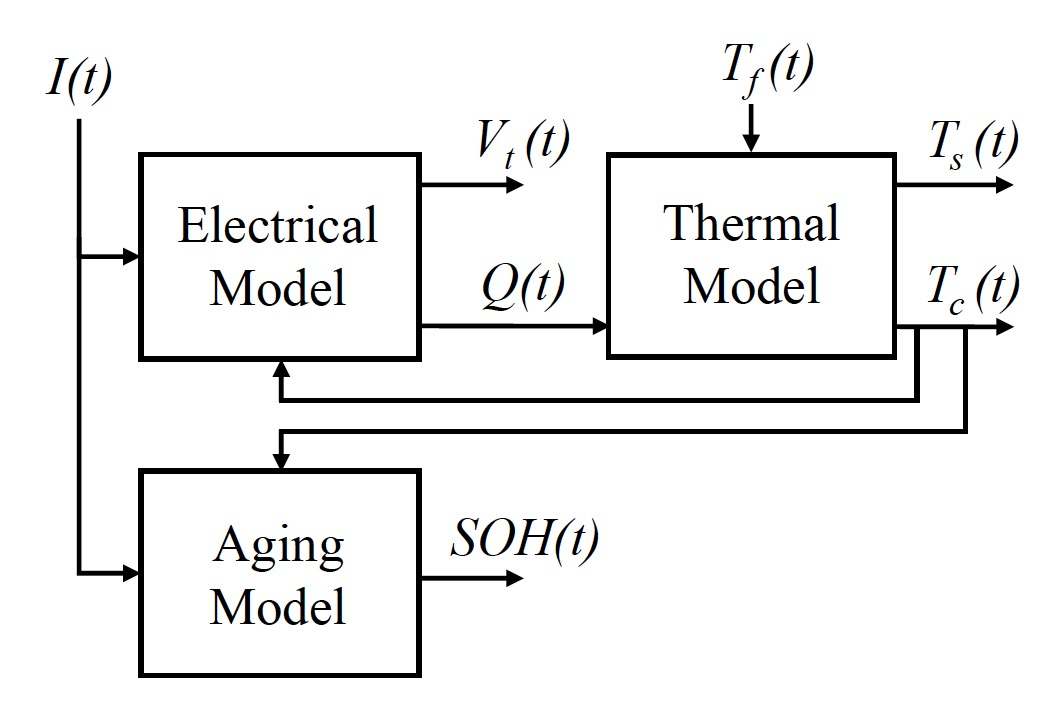
\includegraphics[height=0.3\textwidth]{coupling.jpg}
	\caption{Electro-Thermal-Aging Model Coupling}
	\label{p2}
\end{figure}
\noindent Combining the above three subsystems, the model dynamics are summarized as below.
\begin{equation}
\frac{\mathrm{d} SOC}{\mathrm{d}t}(t) = \frac{I(t)}{C_{bat}}
\end{equation}
\begin{equation}
\frac{\mathrm{d} V_1}{\mathrm{d}t}(t) = -\frac{V_1(t)}{R_1C_1}+\frac{I(t)}{C_1}
\end{equation}
\begin{equation}
\frac{\mathrm{d} V_2}{\mathrm{d}t}(t) = -\frac{V_2(t)}{R_2C_2}+\frac{I(t)}{C_2}
\end{equation}
\begin{equation}
\frac{\mathrm{d}T_c(t)}{\mathrm{d} t} = \frac{T_s(t)-T_c(t)}{R_cC_c}+\frac{I(t)(V_1(t)+V_2(t)+R_0I(t)}{C_c}
\end{equation}
\begin{equation}
\frac{\mathrm{d}T_s(t)}{\mathrm{d} t} = \frac{T_f(t)-T_s(t)}{R_uC_s}+\frac{T_s(t)-T_c(t)}{R_cC_s}
\end{equation}
\begin{equation}
\frac{\mathrm{d} SOH}{\mathrm{d}t}(t) = -\frac{|I(t)|}{2N(c, T_c) C_{bat}}
\end{equation}
\noindent Inputs in this model include current $I_(t)$, which is controllable, and ambient temperature $T_f(t)$, which is uncontroable. 
In our simulation, the input current is a pulse current in a period of 700s, as is shown in \ref{fig:input}, which remains zero for 100s in each period. Besides, he ambient temperature is set to be a sine wave to test the results, as shown below.
\begin{equation}
	T_f(t) = 23.15+\sin( 2\pi\frac{t}{T})
\end{equation}
where $T$ is the duration of our simulation. 
\begin{figure}[H]
	\centering
	\begin{subfigure}[t]{0.4\textwidth}
		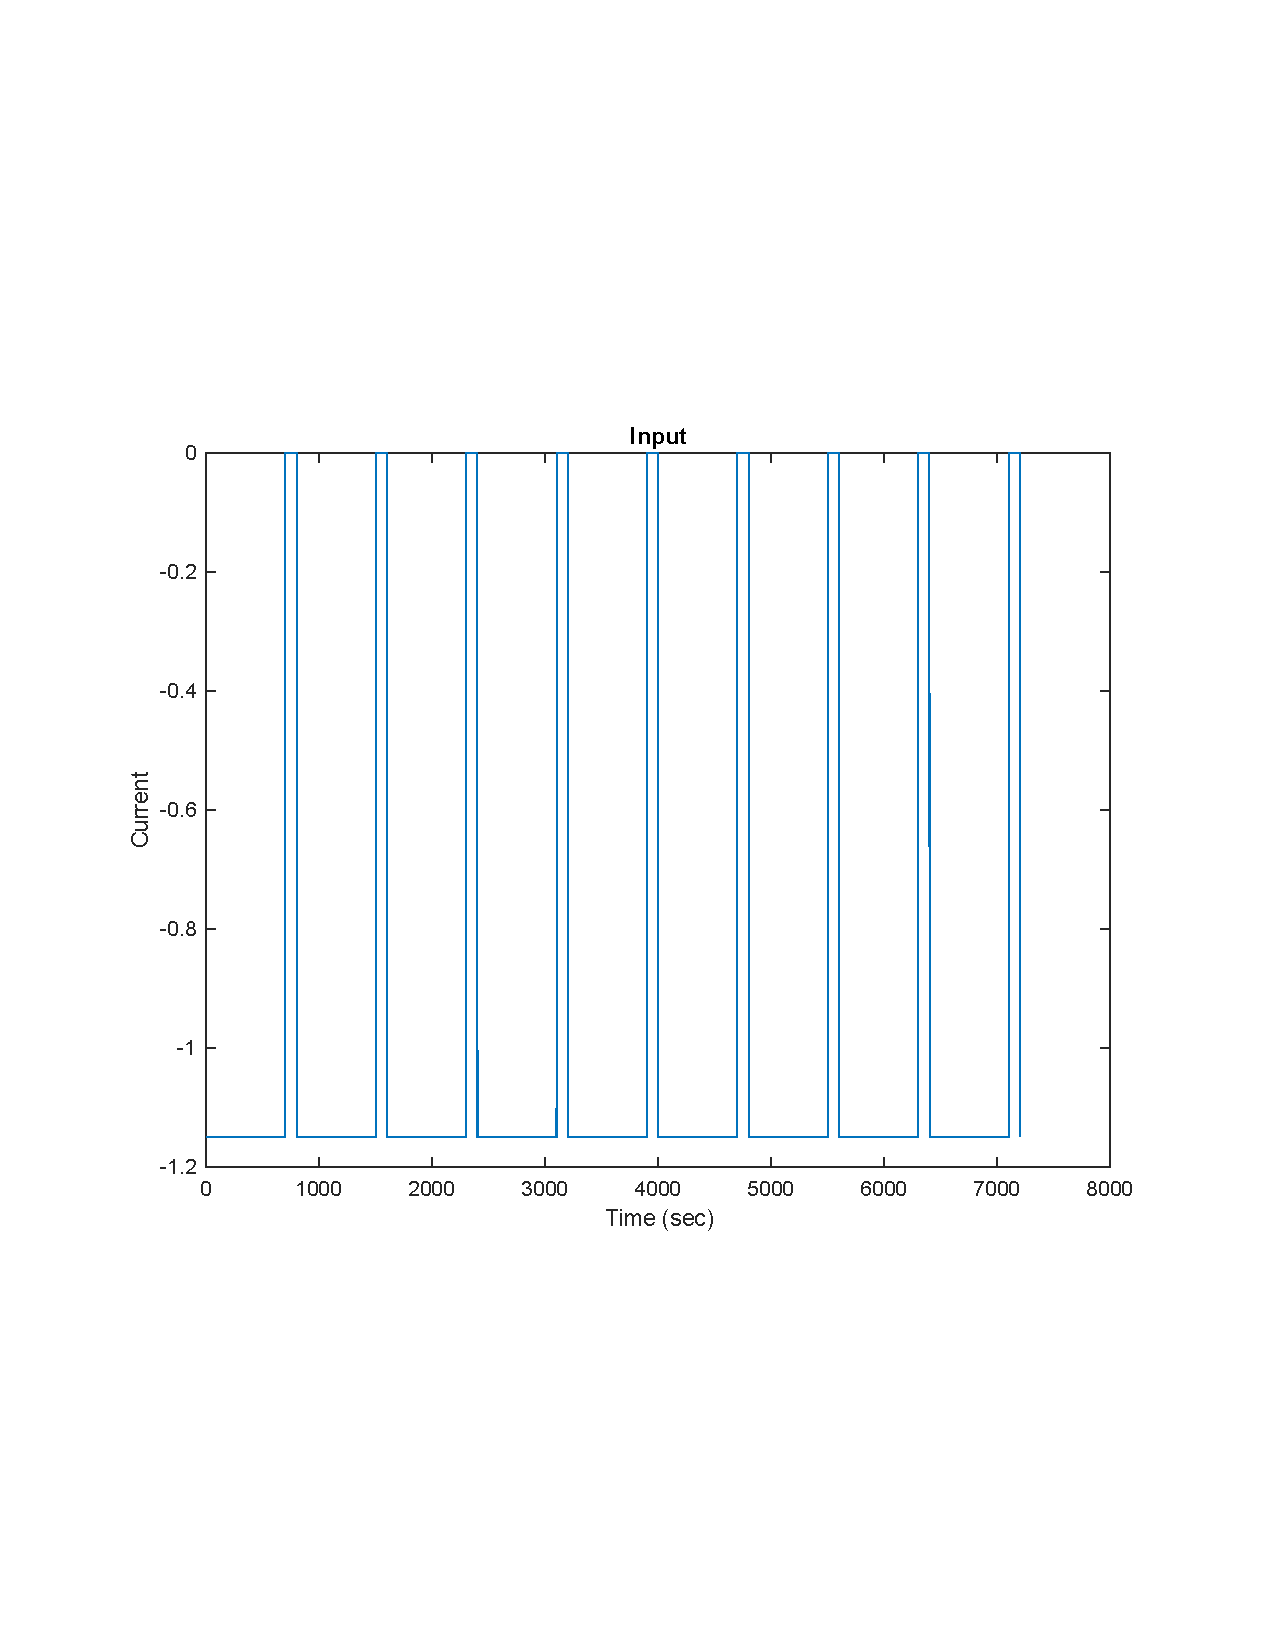
\includegraphics[width=\textwidth]{current.pdf}
		\caption{Time vs. input current}
		\label{fig:inputCurrent}
	\end{subfigure}
	\begin{subfigure}[t]{0.4\textwidth}
		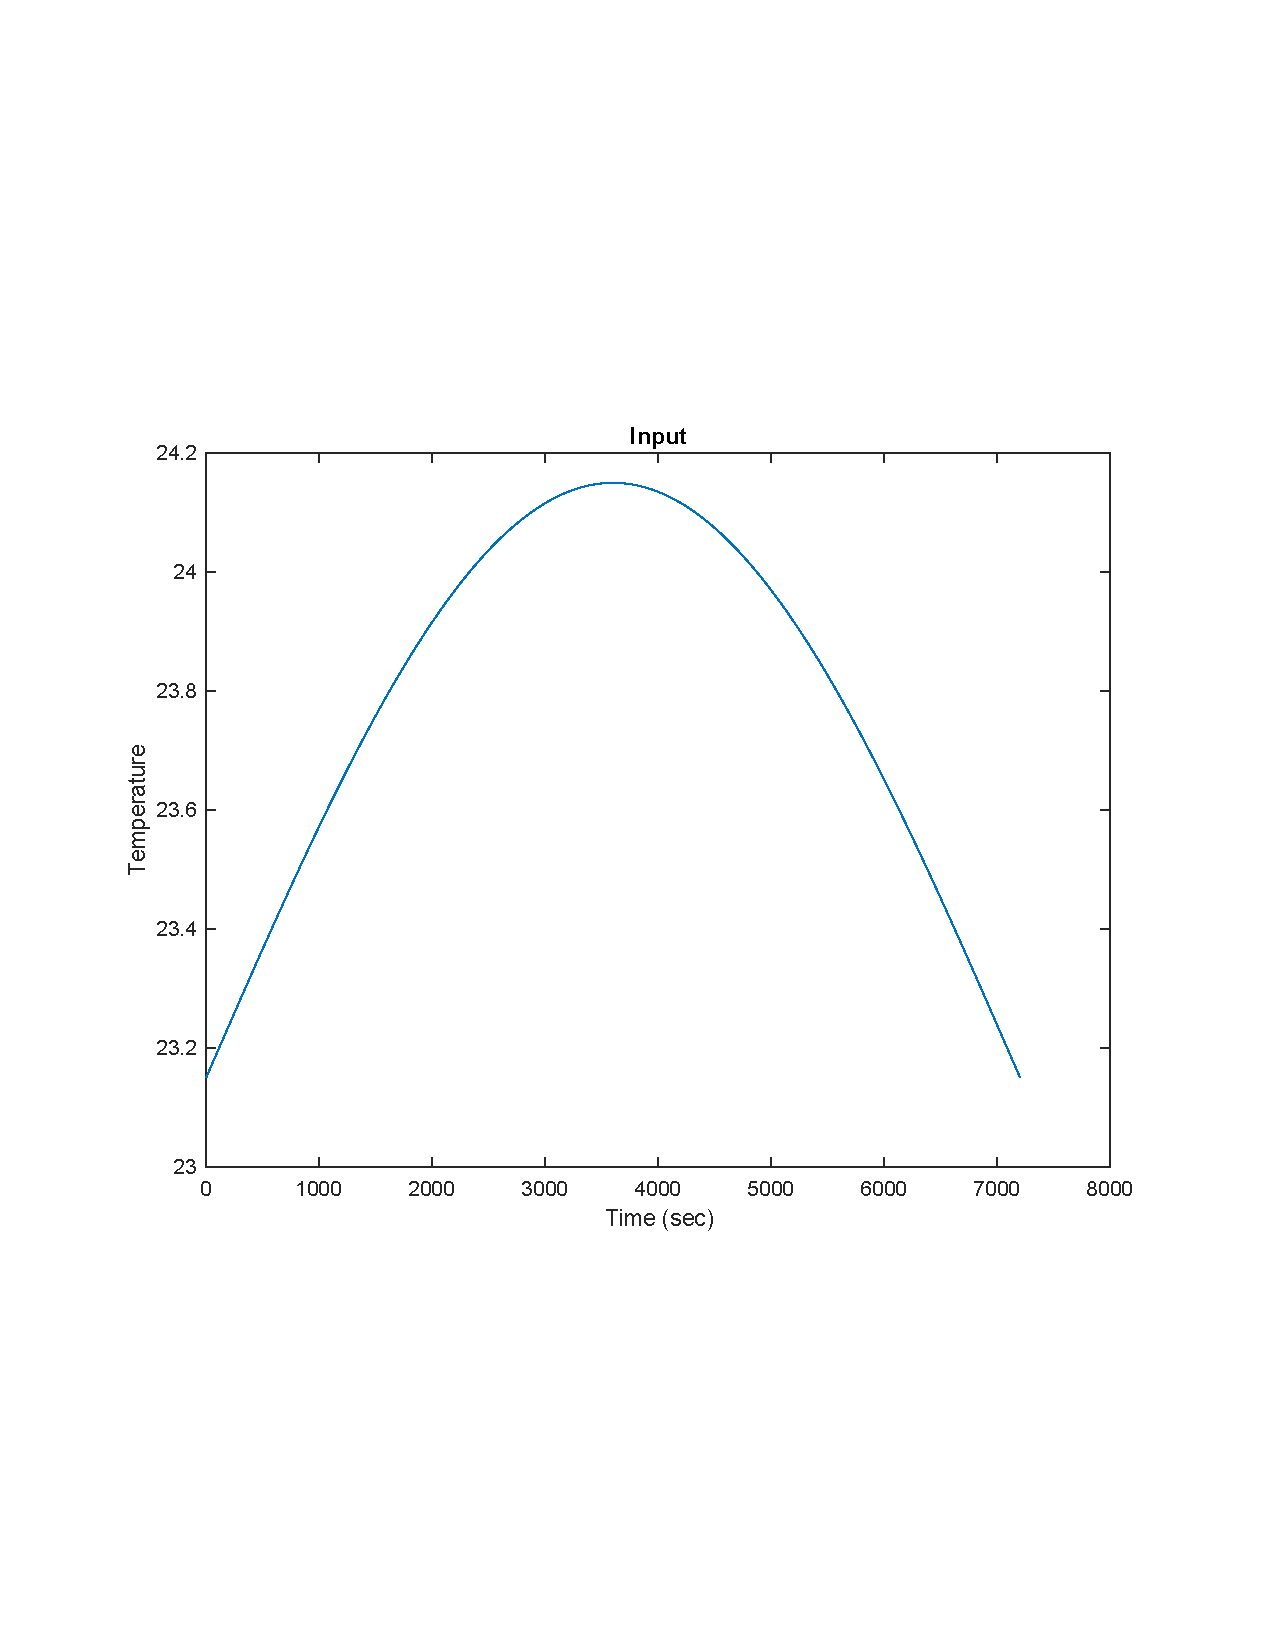
\includegraphics[width=\textwidth]{temperature.pdf}
		\caption{Time vs. input temperature}
		\label{fig:inputTempr}
	\end{subfigure}

	\caption{Input of the simulation}\label{fig:input}
\end{figure}
\noindent Our outputs include the state-of-charge $SOC$, State-of-Health $SOH$, core temperature $T_c$ and surface temperature $T_s$ of the battery.
\section{Discussion}
The simulation result is shown in Figure~\ref{fig:sim}.
\begin{figure}[H]
	\centering
	\begin{subfigure}[t]{0.36\textwidth}
		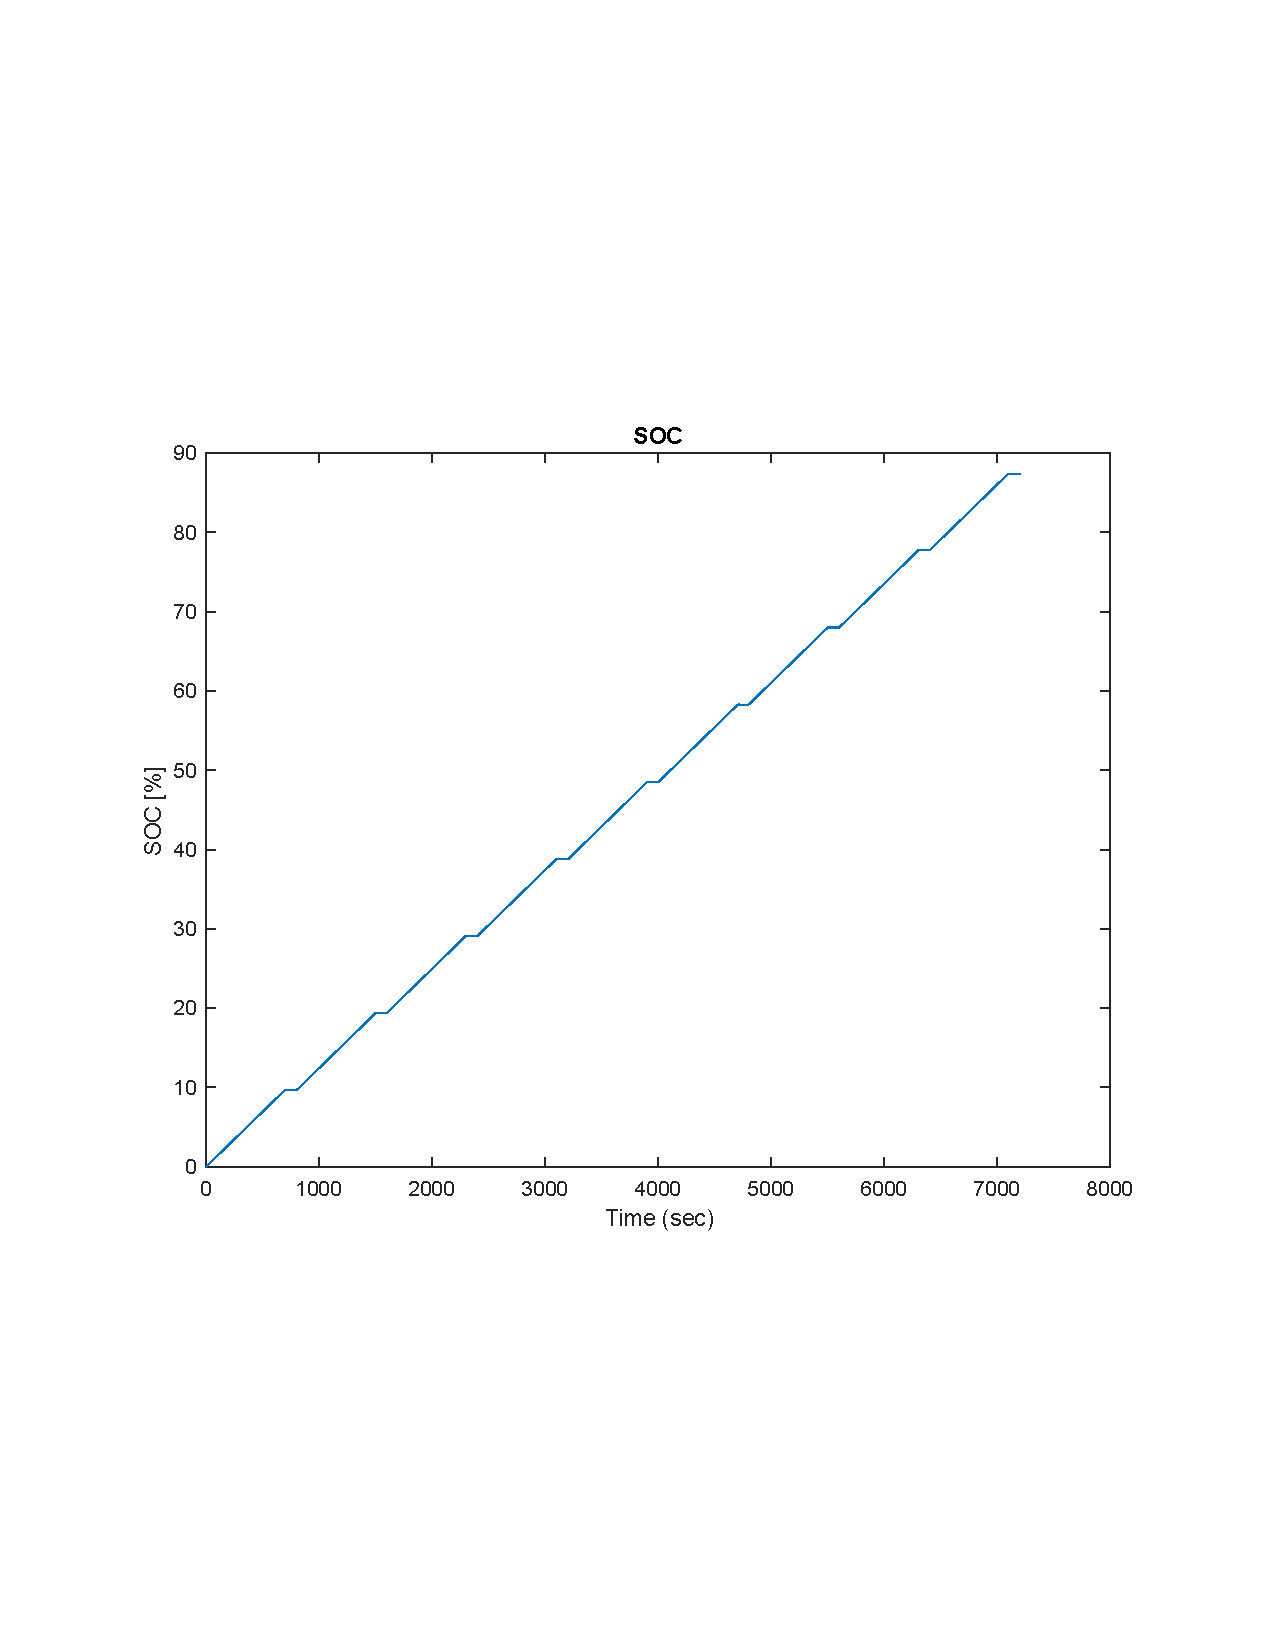
\includegraphics[width=\textwidth]{SOC.pdf}
		\caption{Time vs. SOC}
		\label{fig:SOC}
	\end{subfigure}
	\begin{subfigure}[t]{0.36\textwidth}
		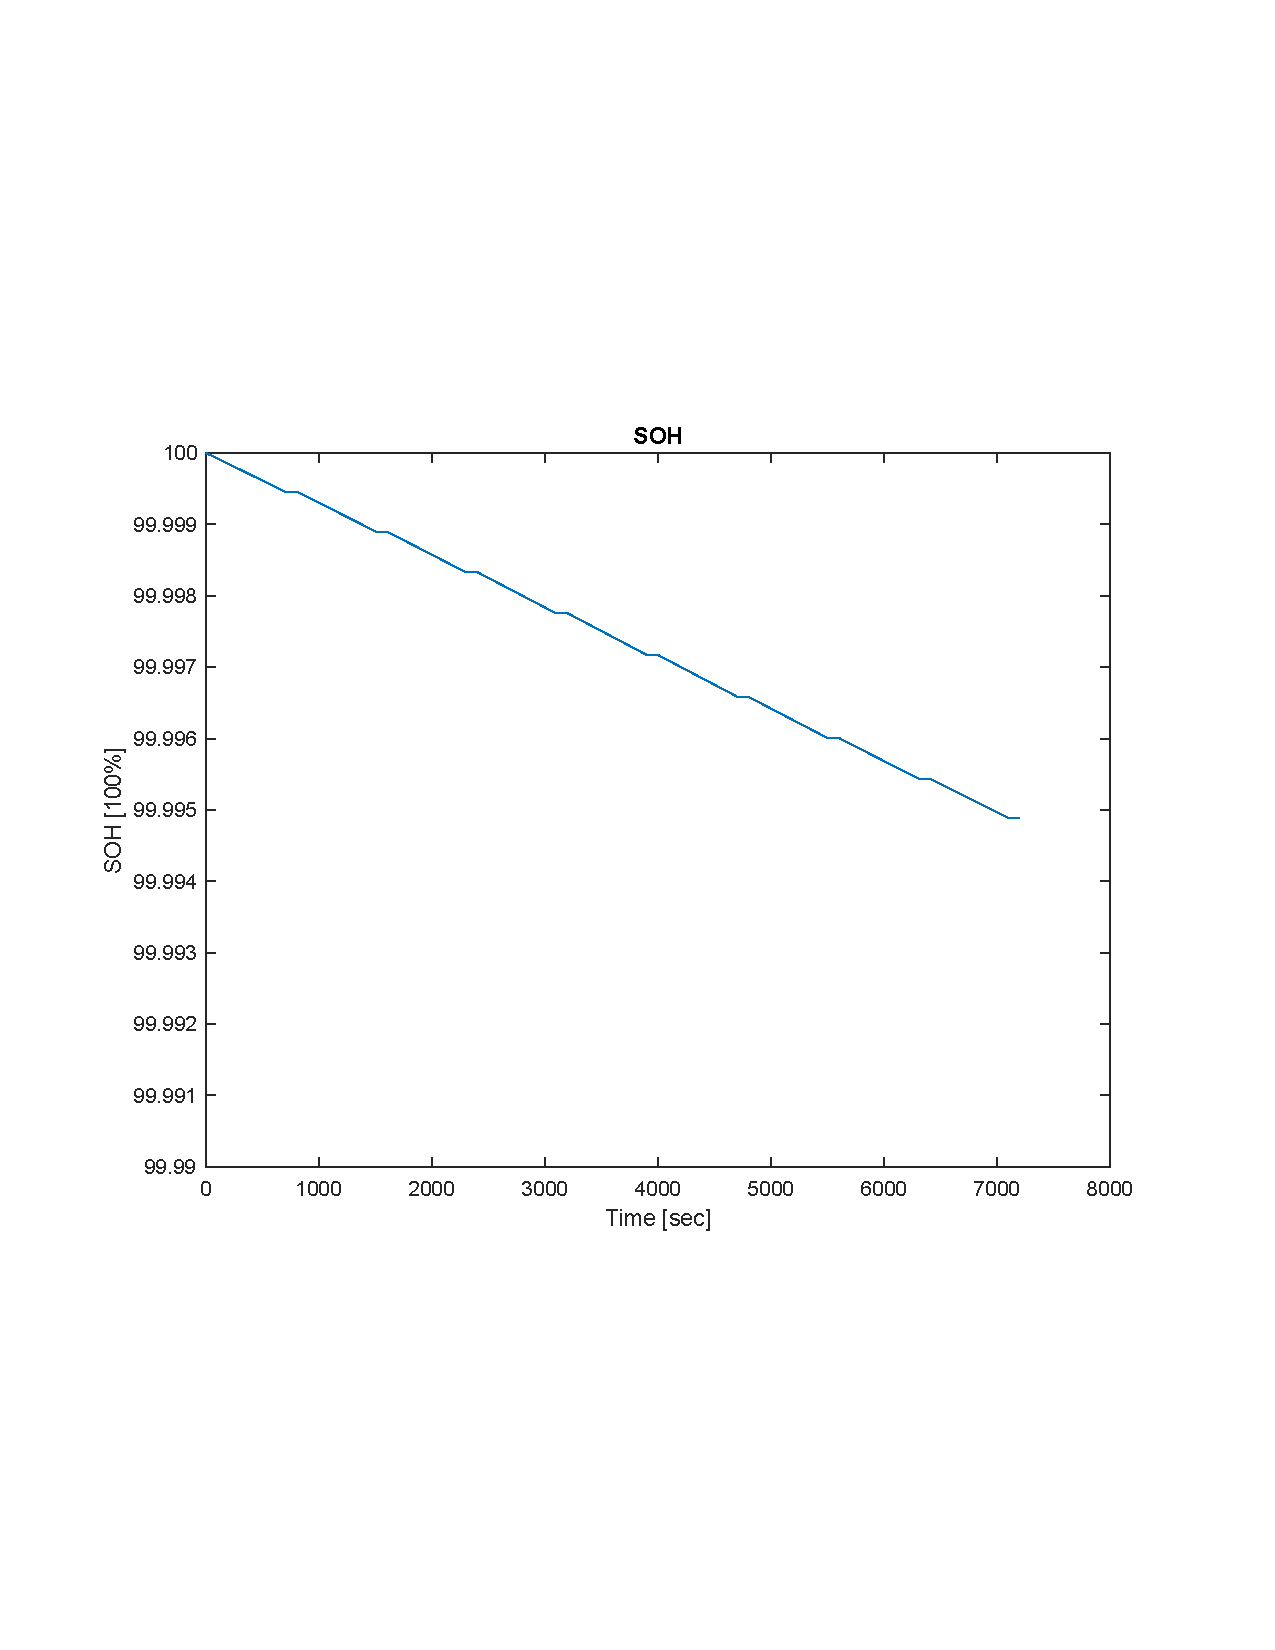
\includegraphics[width=\textwidth]{SOH.pdf}
		\caption{Time vs. SOH}
		\label{fig:SOH}
	\end{subfigure}
	\begin{subfigure}[t]{0.36\textwidth}
		\includegraphics[width=\textwidth]{tempchange.pdf}
		\caption{Time vs. temperature change}
		\label{fig:tempChange}
	\end{subfigure}
	\vspace{-0.25cm}
	\caption{Simulation result}\label{fig:sim}
\end{figure}
\noindent From Figure~\ref{fig:sim} we notice that SOC has a positive linear relationship with charging time while SOH has a negative linear relationship with charging time. In our simulation, It requires nearly 2 hours to replenish the SOC from 0\% to 90\%, with the associated 0.005\% SOH decay. The highest SOC is 87.4\%, and the lowest SOH is 99.995\% compared to the original status. Such a result indicates that charge time and battery health is a trade off, just as we have expected. In addition, we notice that core temperature and surface temperature have the same trend during the charging process, and the maximum temperature is reached at about a half of the charging period, which is also affected by the ambient temperature. For optimal charging, both temperature and aging dynamics should be considered. We will work on it during the next step.
\section{Summary}
In this report, we built the electrical model, thermal model, and aging model, and implemented the open-loop simulation. The goal of this project is to develop a battery observing system with high efficiency and robustness. Since the open-loop simulation result showed that SOC increases while SOH decreases as time goes by, there is a trade off between charge time and battery capacity fade, which perfectly aligns with what we have expected. Both core and surface temperature have a peak in the charging process, which could provide a useful guide if we would like to control the temperature in case that it would reach the safety threshold. However, all of our current conclusions were obtained from simulations, not actual tests. To be more convincing and to refine our model, real-word data is needed and experiment should be implemented. \textbf{Hence, future work will focus on the real-work data implementation. Model accuracy will be tested using Luenberger observer and Kalman filter.} 
\begin{thebibliography}{9}
\bibitem{ref:1} 
Perez, Hector Eduardo, et al.
``Optimal Charging of Li-Ion Batteries With Coupled Electro-Thermal-Aging Dynamics." 
\textit{IEEE Transactions on Vehicular Technology}. 
66.9 (2017): 7761-7770.
\bibitem{ref:2}
Perez, Hector E., et al.
``Parameterization and validation of an integrated electro-thermal cylindrical lfp battery model."
\textit{ASME 2012 5th Annual Dynamic Systems and Control Conference joint with the JSME 2012 11th Motion and Vibration Conference}. 
American Society of Mechanical Engineers, 2012.
\bibitem{ref:3}
Wang, John, et al. 
``Cycle-life model for graphite-LiFePO4 cells." \textit{Journal of Power Sources}
196.8 (2011): 3942-3948.
\end{thebibliography}
\end{document}